\documentclass[runningheads]{llncs}

\usepackage[T1]{fontenc}
\usepackage{graphicx}
\usepackage{amsmath}
\usepackage{amssymb}
\usepackage{tikz}
\usetikzlibrary{arrows.meta,positioning,fit,calc}
\usepackage{caption}
\usepackage{subcaption}
\usepackage{booktabs}
\usepackage{hyperref}

\graphicspath{{figures/}}

\begin{document}

\title{Pattern Layout Optimization for Seam-Aware Texture Alignment}

\author{
    First Author\inst{1} \and
    Second Author\inst{2}
}

\authorrunning{F. Author et al.}

\institute{
    Institute One, City, Country \email{first@example.com} \and
    Institute Two, City, Country \email{second@example.com}
}

\maketitle

\begin{abstract}
Placing 2D garment panels on a fabric roll efficiently is a well-studied
combinatorial optimisation problem, yet existing methods treat the fabric
texture as irrelevant and ignore whether periodic patterns such as stripes
or checks align across the seams of the assembled garment.
Prior work on texture alignment assumes an unbounded fabric supply and
operates by directly deforming 2D patch shapes, leaving fit changes implicit
and unmeasured.
We propose a joint optimisation framework that simultaneously minimises
fabric consumption, seam-wise texture misalignment, and garment fit
deviation.
Seam positions are optimised directly on the 3D body mesh, so that fit
changes are grounded in 3D geometry and can be explicitly measured and
minimised.
We model the periodic structure of the fabric via wallpaper symmetry groups,
supporting a range of patterns including those with glide-reflection symmetry
such as herringbone, chevron, and brick bond.
The problem is solved with a genetic algorithm that accommodates the mixed
nature of the genotype: continuous seam parameters, discrete orientation and
phase offsets, and a combinatorial nesting order, each with dedicated
crossover and mutation operators.
We introduce three baselines and evaluate the method on three garment types
with layouts of up to 400 pattern pieces.
Qualitative and quantitative comparisons against the baselines demonstrate
the benefit of the genetic algorithm and show scalability and robustness
across garment categories.
\keywords{garment pattern nesting \and texture alignment \and evolutionary algorithm \and wallpaper groups \and seam optimisation}
\end{abstract}

\section{Introduction}
\label{sec:introduction}

The global apparel industry generates substantial fabric waste,
a significant portion of which arises from inefficient placement of 2D garment
panels (commonly called \emph{pattern pieces}) on the fabric roll prior
to cutting.
The task of arranging these panels to minimise wasted material is known as
\emph{nesting} (or \emph{marker making}), and has been extensively studied as
a combinatorial optimisation problem~\cite{BennellO08}.
Classical nesting methods, as well as the prevailing industry standard,
treat texture as irrelevant: panels are placed purely for compactness,
with no regard for whether the fabric pattern (stripes, checks, herringbone,
or other periodic motifs) continues seamlessly across the seams of the
assembled garment.

The problem of aligning periodic textures along garment seams has been
addressed by Wolff et al.~\cite{WolffS19}, who directly deform
the 2D patch shapes to achieve alignment.
Their formulation, however, assumes an unbounded fabric supply: roll width and
material efficiency play no role, so the method is decoupled from the
practical nesting problem.
Furthermore, by operating directly on 2D patch geometry, fit changes induced
by the deformation are implicit and go unmeasured. There is no mechanism
to bound or quantify how much the modified pattern deviates from the
originally designed garment.

We argue that seam placement is best optimised in 3D, on the body surface,
rather than by deforming flat patches.
Moving a seam line on the body mesh changes the 2D pattern only as a
consequence of flattening, keeping the modification grounded in 3D geometry.
Critically, this makes fit deviation explicit: the difference between
the flattened and the original 3D surface can be directly measured and
minimised as part of the optimisation.
We formalise this observation and build on it to define a joint optimisation
problem that simultaneously addresses fabric efficiency, seam-aware texture
alignment, and fit preservation, objectives that have not previously been
considered together.

\paragraph{Contributions.}
\begin{enumerate}
    \item We formulate garment pattern layout as a joint optimisation over
          seam positions, fabric efficiency, and texture alignment under
          realistic fabric roll constraints, the first method to address
          all three objectives simultaneously.

    \item We propose a 3D-grounded seam optimisation paradigm in which fit
          deviation is an explicit, measurable objective. In contrast to prior
          2D patch deformation approaches, fit change is no longer implicit
          and unmeasured.

    \item We support texture alignment across a set of wallpaper symmetry
          classes, including patterns with glide-reflection symmetry such as
          herringbone, chevron, and brick bond.

    \item We demonstrate scalability to layouts of up to TODO pattern pieces
          and robustness across TODO garment types (shirts, pants, onesies,
          and dresses).
\end{enumerate}

\paragraph{Outline.}
Section~\ref{sec:related_work} reviews related work on nesting, texture
alignment, and evolutionary approaches to garment optimisation.
Section~\ref{sec:method} presents the problem formulation and the full
optimisation pipeline.
Section~\ref{sec:experiments} reports experimental results.
Section~\ref{sec:conclusion} concludes.

\section{Related Work}
\label{sec:related_work}

% ---------------------------------------------------------------------------
\subsection{Garment Pattern Nesting}
\label{sec:rw_nesting}

The problem of placing irregularly shaped panels on a strip to minimise
wasted material is known as the irregular strip packing or nesting
problem~\cite{WascherHS07}.
Bennell and Oliveira~\cite{BennellO08} provide a comprehensive tutorial
covering the principal geometric tools, from raster methods to the
no-fit polygon (NFP), and Le{\~a}o et al.~\cite{LeaoTOCA20} give a recent
review of mathematical models for irregular packing.
The NFP, which characterises all valid non-overlapping placements of one
polygon relative to another, underpins many state-of-the-art nesting
solvers~\cite{BurkeHKW07}.
Burke et al.~\cite{BurkeHKW06} introduce the bottom-left-fill (BLF)
heuristic, which places each piece at the lowest, leftmost feasible position
on the strip; Mart{\'i}nez-Sykora et al.~\cite{MartinezSykoraACRO22}
recently proposed a fast, scalable BLF variant based on a semi-discrete
representation.
Our nesting engine builds on the classical BLF paradigm.

Metaheuristic approaches have been widely applied to nesting.
Jakobs~\cite{Jakobs96} introduces one of the first genetic algorithm
formulations for polygon packing, encoding placement order as a permutation.
Mundim et al.~\cite{MundimAQO17} apply a biased random-key genetic
algorithm to open-dimension nesting with a no-fit raster representation.
Heckmann and Lengauer~\cite{HeckmannL95} address the textile industry
specifically with simulated annealing, and
Gomes and Oliveira~\cite{GomesO06} combine simulated annealing with linear
programming for local compaction.
Elkeran~\cite{Elkeran13} achieves strong results with guided cuckoo search
and pairwise clustering.

All of the above methods treat texture as irrelevant: panels are placed
purely for geometric compactness with no regard for pattern continuity
across seams.
NFP-based solvers represent the state of the art for fabric efficiency
alone; our nesting component uses a BLF heuristic since the novelty lies
in the joint objectives, and any NFP-based engine could be substituted
without affecting the other contributions.

% ---------------------------------------------------------------------------
\subsection{Texture and Pattern Alignment}
\label{sec:rw_texture}

Ko and Kim~\cite{Ko2013} address nesting on figured (patterned) fabric using
image analysis and 3D drape simulation to preserve figure continuity across
pieces.
Their approach jointly considers placement and pattern matching, but is
limited to simple repeat patterns and does not handle the full symmetry
structure of periodic textures.

Wolff and Sorkine-Hornung~\cite{WolffS19} present the most comprehensive
prior work on seam-aware texture alignment in garments.
They formalise the alignment problem using all 17 wallpaper groups and
optimise the placement of sewing pattern pieces to minimise phase mismatch
along seams, with optional deformation of the seam shapes themselves.
A follow-up~\cite{WolffHS19} extends this framework to enforce body
reflection symmetry constraints on both texture alignment and seam shape.
While this line of work establishes the formal foundations for wallpaper
group alignment, it assumes an unbounded fabric supply and ignores material
efficiency entirely.
Furthermore, by operating directly on 2D patch geometry, any deformation
introduced to improve alignment implicitly modifies the garment fit, with
no mechanism to measure or bound this change.

Pietroni et al.~\cite{PietroniDFLVS22} address a complementary problem:
given a 3D garment shape, they segment it into panels and compute 2D
parameterizations that respect tailoring constraints such as seam symmetry,
dart placement, and fabric grain alignment, with a flattening distortion
measure that models woven-fabric deformation.
Their objective is to optimise seam placement for minimal flattening
distortion, whereas our method optimises seam placement for texture
alignment under fabric roll constraints.


% ---------------------------------------------------------------------------
\subsection{Multi-Objective Evolutionary Algorithms and Mixed-Type Genotypes}
\label{sec:rw_moea}

The seminal NSGA-II algorithm~\cite{Deb2002NSGAII} establishes the standard
framework for Pareto-based multi-objective optimisation with tournament
selection: candidate solutions are compared by dominance, with a
crowding-distance tiebreaker to maintain diversity.
Deb and Jain~\cite{DebJ14} extend this to many-objective problems in
NSGA-III with reference-point-based selection.
We adopt a simplified variant of the NSGA-II selection scheme, using
fitness sum as the tiebreaker in place of crowding distance, which is
sufficient for our three-objective problem.

The mixed structure of our genotype (continuous seam parameters, discrete
orientations and phase offsets, and a combinatorial nesting order) requires
dedicated operators per variable type.
Michalewicz~\cite{Michalewicz1996} establishes the foundational treatment
of mixed-type chromosomes in evolutionary computation, arguing that each
variable type benefits from operators that respect its domain structure.
Li et al.~\cite{LiEEBSDR13} formalise this principle in Mixed Integer
Evolution Strategies (MIES), defining separate self-adaptive mutation
operators for continuous, integer, and nominal discrete variables within
a unified algorithm.
Our design follows this principle, as detailed in Section~\ref{sec:ea}.

\section{Method}
\label{sec:method}

We formulate garment pattern layout as a mixed-type optimisation problem
and solve it with a multi-objective genetic algorithm.
The pipeline maps a genotype encoding seam positions, patch orientations,
texture phase offsets, and nesting parameters to a fabric layout,
which is then scored by three objectives: fabric efficiency,
texture alignment across seams, and garment fit quality.

% ---------------------------------------------------------------------------
\subsection{Problem Formulation}
\label{sec:formulation}

We define the problem as
\[
\Psi = \langle M, \mathcal{T}, \mathcal{L}, \mathbf{w}, \Omega \rangle,
\]
where $M = (V, E, F)$ is the 3D garment mesh,
$\mathcal{T}$ is a periodic fabric texture characterised by a lattice basis
$B = \{\mathbf{u}, \mathbf{v}\}$,
$\mathcal{L} = \{L_1, \dots, L_m\}$ is a set of admissible quad regions on
the mesh surface that constrain where seam keypoints may be placed,
$\mathbf{w} = \{w_s\}_{s \in \mathcal{S}}$ are static per-seam importance
weights ($w_s \in [0,1]$, set to zero for boundary seams),
and $\Omega = [0, W] \times [0, \infty)$ is the fabric roll domain of
width $W$.

% ---------------------------------------------------------------------------
\subsection{Texture Symmetry: Wallpaper Groups}
\label{sec:wallpaper}

The periodic structure of a fabric texture is fully characterised by its
wallpaper group $\mathcal{G}$, which encodes all translational, rotational,
and reflective symmetries of the pattern.
Accounting for $\mathcal{G}$ is essential for two reasons.
First, it constrains which grain-rotation pairs $(\rho_i, \rho_j)$ of adjacent
patches can produce a valid seam alignment: for a stripe pattern, rotating one
patch by 90° makes alignment impossible regardless of placement.
Second, patterns with glide-reflection symmetry (e.g.\ herringbone, chevron)
allow patches to align via a reflected copy of the texture, which must be
accounted for in the mismatch computation.

We support eight groups, summarised in Table~\ref{tab:wallpaper}.

\begin{table}[t]
\centering
\caption{Supported wallpaper groups with seam compatibility rules.}
\label{tab:wallpaper}
\begin{tabular}{llll}
\toprule
Group & Name & Pattern & Seam compatibility \\
\midrule
PM  & stripes          & horizontal stripes    & $\rho_i \equiv \rho_j \pmod{2}$ \\
PM  & diagonal stripes & stripes at 45°        & $\rho_i \equiv \rho_j \pmod{2}$ \\
PMM & grid             & check / plaid         & all pairs \\
P4  &                  & 4-fold rotation       & all pairs \\
P4M &                  & 4-fold + mirrors      & all pairs \\
PG  & herringbone      & glide reflection only & $\rho_i \equiv \rho_j \pmod{2}$ \\
PMG & chevron          & mirror + glide        & $\rho_i \equiv \rho_j \pmod{2}$ \\
PGG & brick bond       & two glide axes        & $\rho_i \equiv \rho_j \pmod{2}$ \\
\bottomrule
\end{tabular}
\end{table}

If $\mathcal{G}$ declares $(\rho_i, \rho_j)$ incompatible, the pair receives
a hard penalty in $f_2$.
For groups with glide-reflection symmetry (PG, PMG, PGG), each group defines
glide maps $\mathcal{G}_s = \{g_1, \dots\}$ acting on fractional phase
coordinates, and the per-point mismatch takes the minimum over the identity
and all glide images:
\[
\Delta_{\mathcal{G}}(\boldsymbol{\phi}_a, \boldsymbol{\phi}_b)
= \min\!\Bigl(
    \Delta(\boldsymbol{\phi}_a, \boldsymbol{\phi}_b),\;
    \min_{g \in \mathcal{G}_s} \Delta(\boldsymbol{\phi}_a, g(\boldsymbol{\phi}_b))
  \Bigr).
\]
For groups without glide symmetry, $\mathcal{G}_s = \emptyset$ and
$\Delta_{\mathcal{G}} = \Delta$.

% ---------------------------------------------------------------------------
\subsection{Genotype: Decision Variables}
\label{sec:genotype}

A candidate solution is encoded as
\[
\mathbf{x} =
\langle
\boldsymbol{\delta},\,
\boldsymbol{\rho},\,
\boldsymbol{\kappa},\,
\pi,\,
h,\,
\lambda_s
\rangle.
\]

\paragraph{Seam topology ($\boldsymbol{\delta}$).}
Each landmark region $L_j$ is a topological quad on the mesh surface defined
by four corner vertices.
The position of seam keypoint $k_j$ within $L_j$ is controlled by a 2D
parameter:
\[
k_j = \Gamma_j(\boldsymbol{\delta}_j), \quad
\boldsymbol{\delta}_j = (u_j, v_j) \in [0,1]^2,
\]
where $\Gamma_j$ performs bilinear interpolation within $L_j$ followed by a
snap to the nearest mesh vertex.
The full vector $\boldsymbol{\delta} \in [0,1]^{2m}$ concatenates all
landmark coordinates.
Seams $s \in \mathcal{S}$ are computed as geodesics between corresponding
keypoints.
Restricting keypoints to semantically defined regions prevents degenerate cuts
while still allowing the EA to explore meaningful seam placements.

\paragraph{Fabric orientation ($\boldsymbol{\rho}$).}
Cutting along seams yields $n$ 2D charts $P(\boldsymbol{\delta}) = \{p_1, \dots, p_n\}$.
Each chart is assigned a discrete grain orientation
\[
\rho_i \in \{0,1,2,3\}, \quad \theta_i = \rho_i \frac{\pi}{2},
\]
which determines how the chart is rotated on the fabric roll.
Compatibility with $\mathcal{G}$ is enforced at evaluation time.

\paragraph{Texture phase offsets ($\boldsymbol{\kappa}$).}
Because the fabric texture repeats periodically, placing a chart at different
positions that are integer multiples of the period apart produces
indistinguishable results.
We exploit this freedom by assigning each chart a discrete phase bin
\[
\kappa_i \in \{0,1,\dots,K-1\},
\]
where $K$ is the number of bins per period.
The bin determines a fractional offset $\kappa_i / K$ applied uniformly along
both lattice axes, effectively choosing which repeat of the texture the chart
is placed on.
Optimising $\boldsymbol{\kappa}$ allows the EA to align stripe or grid bands
across seams without moving the patches on the fabric.

\paragraph{Parameterization hyperparameter ($\lambda_s$).}
The seam straightness weight
\[
\lambda_s \in \{2^0, 2^1, \dots, 2^7\}
\]
controls the strength of the regularization term in the parameterization
energy that encourages seam boundaries to be straight lines in 2D.
It is applied uniformly across all seams.

\paragraph{Nesting variables ($\pi, h$).}
The permutation $\pi \in S_n$ defines the order in which charts are placed
on the fabric, and $h \in \mathcal{H}$ ($|\mathcal{H}|=3$) selects the
bottom-left placement heuristic variant.

% ---------------------------------------------------------------------------
\subsection{Phenotype: From Genotype to Layout}
\label{sec:phenotype}

\subsubsection{Seam Cutting and Parameterization.}
Given $\boldsymbol{\delta}$, the keypoints $\{k_j\}$ are computed via
bilinear interpolation and snapped to mesh vertices.
Geodesic paths between corresponding keypoints define the seam network,
along which the mesh is cut to yield 3D patches.
Each patch is then flattened to 2D by LSCM parameterization, with a
seam-straightness regularization weighted by $\lambda_s$.

\subsubsection{Stage 2: Global Phase Alignment.}
\label{sec:stage2}
After parameterization, patches connected by seams with $w_s > 0$ form
connected components.
Within each component a small translational correction $\mathbf{c}_i \in \mathbb{R}^2$
is found per patch (root fixed at $\mathbf{c}_i = \mathbf{0}$) by minimising
the total seam phase residual:
\[
C = \sum_{\substack{s \in \mathcal{S} \\ w_s > 0}}
    w_s \sum_{(a,b) \in s} \left\|\mathbf{r}_{ab}\right\|^2,
\]
where the signed wrapped residual per axis is
\[
r^d_{ab}
= \mathrm{wrap}\!\left(
    \mathrm{Phase}_i(\mathbf{x}_a + \mathbf{c}_i)^d
  - \mathrm{Phase}_j(\mathbf{x}_b + \mathbf{c}_j)^d
\right), \quad d \in \{u,v\},
\]
and $\mathrm{wrap}(\cdot)$ maps to $[-\tfrac{1}{2},\tfrac{1}{2})$.
This is solved with Levenberg--Marquardt using finite-difference Jacobians.
The corrections are baked into the patch vertices before nesting.

\subsubsection{Nesting.}
Each chart is rotated by $R(\theta_i)$ and placed on the fabric roll using
heuristic $h$ in order $\pi$.
Placements are snapped to the texture lattice so that the absolute position
on the roll does not introduce an uncontrolled phase offset.
Charts must satisfy non-overlap and containment constraints:
\begin{align}
(\phi_i(p_i) + \mathbf{t}_i) \cap (\phi_j(p_j) + \mathbf{t}_j) &= \emptyset, \\
(\phi_i(p_i) + \mathbf{t}_i) &\subset \Omega.
\end{align}

% ---------------------------------------------------------------------------
\subsection{Objective Functions}
\label{sec:objectives}

The fitness vector is
\[
\mathbf{F}(\mathbf{x}) = [w_1 f_1,\; w_2 f_2,\; w_3 f_3]^T,
\]
where $w_1, w_2, w_3 \geq 0$ are designer-specified weights and all three
components are minimised.

\paragraph{Fabric efficiency ($f_1$).}
\[
f_1(\mathbf{x}) = \frac{1}{W} \max_{p \in \text{Layout}} y_{\max}(p).
\]
Normalising by $W$ makes $f_1$ dimensionless and comparable to $f_2$
regardless of the physical scale of the fabric.

\paragraph{Texture alignment ($f_2$).}
The 2D lattice phase of a fabric point $\mathbf{x}$ is
\[
\mathrm{Phase}(\mathbf{x}) = \mathrm{frac}([B]^{-1}\mathbf{x}) \in [0,1)^2,
\]
where $[B] = [\mathbf{u} \mid \mathbf{v}]$ and $\mathrm{frac}(\cdot)$ is
applied component-wise.
For chart $p_i$, the kappa offset shifts the phase uniformly:
\[
\mathrm{Phase}_i(\mathbf{x}) =
\mathrm{frac}\!\left(\mathrm{Phase}(\mathbf{x}) + \frac{\kappa_i}{K}\mathbf{1}\right),
\quad \mathbf{1} = (1,1)^T.
\]
For stripe groups, the pattern is translation-invariant along the stripe axis,
so that phase component contributes zero to any difference.
The per-point mismatch between two phases is
\[
\Delta(\boldsymbol{\phi}_a, \boldsymbol{\phi}_b)
= \tfrac{1}{2}\bigl(
    \delta^u(\boldsymbol{\phi}_a, \boldsymbol{\phi}_b)
  + \delta^v(\boldsymbol{\phi}_a, \boldsymbol{\phi}_b)
\bigr),
\quad
\delta^d = \min\!\left(|\phi_a^d - \phi_b^d|,\; 1 - |\phi_a^d - \phi_b^d|\right).
\]
The seam mismatch integrates this over each seam arc-length:
\[
\mathrm{Mismatch}(s)
= \frac{1}{L_s} \int_0^{L_s}
  \Delta_{\mathcal{G}}\!\bigl(
    \mathrm{Phase}_i(\mathbf{x}_i(l)),\,
    \mathrm{Phase}_j(\mathbf{x}_j(l))
  \bigr)\, dl,
\]
and $f_2$ accumulates this over all seams weighted by importance:
\[
f_2(\mathbf{x}) = \sum_{s \in \mathcal{S}} w_s \cdot \mathrm{Mismatch}(s).
\]

\paragraph{Fit distortion ($f_3$).}
\[
f_3(\mathbf{x}) = \frac{1}{n} \sum_{i=1}^n \overline{\sigma}_i^{\,\mathrm{weft}},
\]
where $\overline{\sigma}_i^{\,\mathrm{weft}}$ is the mean local triangle
stretch deviation along the weft direction between corresponding 2D and 3D
triangles of chart $p_i$.

% ---------------------------------------------------------------------------
\subsection{Evolutionary Algorithm}
\label{sec:ea}

The mixed structure of the genotype — continuous ($\boldsymbol{\delta}$),
discrete ($\boldsymbol{\rho}, \boldsymbol{\kappa}, \lambda_s, h$),
and combinatorial ($\pi$) — motivates a genetic algorithm with
variable-specific operators rather than a standard real-valued EA.

\paragraph{Selection.}
Tournament selection with tournament size $k=3$ is used.
The primary criterion is Pareto dominance: a candidate $\mathbf{x}$ dominates
$\mathbf{y}$ if $\mathbf{F}(\mathbf{x}) \leq \mathbf{F}(\mathbf{y})$
component-wise with at least one strict inequality.
When neither candidate dominates the other, the fallback criterion is the
scalar sum $\sum_i w_i f_i$, which provides a consistent total order
without discarding multi-objective information.

\paragraph{Crossover.}
Applied with probability $p_c$.
Each variable type uses a dedicated operator:
\begin{itemize}
    \item $\boldsymbol{\delta}, \boldsymbol{\rho}, \boldsymbol{\kappa}$:
          uniform gene-wise swap — each gene is exchanged between parents
          independently with probability $\tfrac{1}{2}$.
    \item $\pi$: whole-permutation inheritance — one parent's permutation is
          copied in full (chosen by coin flip) to preserve permutation validity.
    \item $h, \lambda_s$: coin flip between the two parent values.
\end{itemize}

\paragraph{Mutation.}
Applied with probability $p_m$ after crossover.
Each variable type uses a dedicated operator:
\begin{itemize}
    \item $\boldsymbol{\delta}$: Gaussian perturbation
          $\delta_j \leftarrow \mathrm{clip}(\delta_j + \mathcal{N}(0, \sigma_\delta),\,
          \delta_{\min}, \delta_{\max})$,
          where $[\delta_{\min}, \delta_{\max}] \subset [0,1]$ avoids
          geometrically degenerate mesh regions.
    \item $\boldsymbol{\kappa}$: each bin resampled uniformly from
          $\{0,\dots,K{-}1\}$ with per-gene probability $p_\kappa$.
    \item $\boldsymbol{\rho}$: each value resampled from $\{0,1,2,3\}$
          with per-gene probability $p_\rho$.
    \item $\pi$: swap of two randomly chosen positions with probability
          $p_\pi$, preserving permutation validity.
    \item $h$: resampled uniformly from $\mathcal{H}$ with probability $p_h$.
    \item $\lambda_s$: resampled uniformly from $\{2^0,\dots,2^7\}$
          with probability $p_{\lambda}$.
\end{itemize}

\paragraph{Elitism.}
The single best individual (by fitness sum) is carried over unchanged to the
next generation, ensuring monotone improvement of the best solution found.

\section{Experiments}
\label{sec:experiments}

% ---------------------------------------------------------------------------
\subsection{Baselines}
\label{sec:baselines}

We compare against four baselines spanning the mixed-integer search
space our method addresses.
B0, B1, and B2 fix seam positions at the midpoints of their respective
landmark quads ($\boldsymbol{\delta} = 0.5$) and differ only in how they
assign texture phase offsets, covering the full range of
$\boldsymbol{\kappa}$-only strategies from no texture awareness (B0) to
the best budget-matched $\boldsymbol{\kappa}$ assignment (B2).
B3 samples the full joint search space of the GA, $(\boldsymbol{\delta},
\boldsymbol{\kappa})$, at the same evaluation budget as one GA run,
covering the "is structured search necessary" question with uniform
random sampling.
All baselines include Stage~2 global phase alignment
(Section~\ref{sec:stage2}) for a fair comparison.

\paragraph{B3: Random search at matched budget.}
B3 draws uniform random $(\boldsymbol{\delta}, \boldsymbol{\kappa})$
samples from the same distribution as the GA's initial population
($\boldsymbol{\delta}_j \sim \mathcal{U}[0.2, 0.8]$,
$\kappa_i \sim \mathcal{U}\{0, \dots, K{-}1\}$), evaluates each with the
same geometry pipeline, Stage~2 solver, and nesting engine as the GA,
and retains the best-found individual under the same fitness weighting.
The sample count is set equal to the GA's evaluation budget
($\mathrm{pop} \times \mathrm{gens} = 2{,}000$), and because both methods
pay the same $55$--$60\,\%$ infeasibility tax on attempted evaluations
(Section~\ref{sec:ea}), they also face the same effective valid-evaluation
budget. B3 and the GA differ only in how they move through the search
space, so any improvement of the GA over B3 is attributable to selection
pressure concentrating the GA's valid samples near previously-discovered
high-quality regions, which uniform random sampling cannot exploit by
construction.

\paragraph{B2: Optimal phase selection.}
Phase offsets are assigned to minimise total seam phase mismatch without
seam repositioning.
For the pants garment ($M=4$, $K^M = 8^4 = 4{,}096$), this is solved by
exhaustive enumeration.
For the onesie ($M=11$, $K^M = 8^{11} \approx 8.6 \times 10^9$),
exhaustive search is intractable; B2 instead evaluates $5 \times 10^5$
uniformly random $\boldsymbol{\kappa}$ assignments and keeps the best.
B2 serves as the ablation for the $\boldsymbol{\delta}$ component: any
improvement of the GA over B2 on $f_\text{align}$ is attributable to seam
position optimisation.

\paragraph{B1: Greedy phase selection.}
Patches are placed in breadth-first order over the seam adjacency graph.
Each patch's phase offset $\kappa_i$ is chosen greedily from $K$ candidates
to minimise mismatch with already-placed neighbours.
This captures the best texture alignment achievable by a greedy strategy
without global optimisation or seam-position search.

\paragraph{B0: Pure greedy nesting.}
All phase offsets are set to zero ($\boldsymbol{\kappa} = \mathbf{0}$),
patches are placed in descending order of area using the bottom-left heuristic,
and no grain rotation is applied.
This represents the classical industry approach: optimising fabric efficiency
with no texture awareness.

% ---------------------------------------------------------------------------
\subsection{Implementation Details}
\label{sec:implementation}

The GA uses a population of 100 individuals evolved for 20 generations with
elite count 4 and tournament size 4.
Crossover is applied with probability 0.7 and mutation with probability 0.7.
Per-variable mutation rates are: $p_\kappa = 0.35$ (kappa flip),
$p_\rho = 0.15$ (rho flip).
Delta is mutated by Gaussian perturbation with $\sigma_\delta = 0.20$,
clamped to the range $[0.2, 0.8]$ to keep keypoints away from degenerate
mesh regions while still allowing meaningful seam repositioning.
We use $K=8$ phase bins per period.

The fabric roll width is $W = 1{,}500\,\text{mm}$ with a texture period of
$50 \times 50\,\text{mm}$.
Fitness weights are $w_\text{fabric} = 1$, $w_\text{align} = 2.5$, $w_\text{fit} = 10$.
All experiments run $N \in \{5, 10, 25, 50, 100\}$ bodies per roll and are
repeated with 10 independent random seeds; we report mean $\pm$ standard
deviation.
Each fitness evaluation takes approximately 5\,s on a single CPU core
(geometry: ${\sim}$4.5\,s, Stage~2: ${\sim}$0.1\,s, nesting: $<$0.01\,s),
so a full GA run of 2{,}000 evaluations completes in approximately
3 hours.
B2 on the onesie runs its geometry pipeline once and then scores
$5 \times 10^5$ $\boldsymbol{\kappa}$ assignments at fixed
$\boldsymbol{\delta} = 0.5$, inspecting 250$\times$ more configurations
than the GA in a strictly smaller subspace; the GA nonetheless
dominates B2 on $f_\text{align}$ (Section~\ref{sec:results}),
justifying the cost of population-based search over the full joint
space.

% ---------------------------------------------------------------------------
\subsection{Garment Types}
\label{sec:garments}

We evaluate on three garment types spanning a range of topological
complexity (Table~\ref{tab:results_garments}).

\textbf{Onesie with sleeves} (\texttt{onesie\_sleeves}) is our primary
evaluation garment: $M=11$ patches connected by 26 geodesic seams, of
which 16 carry non-zero importance weights.
The combination of torso, legs, and sleeves produces a rich seam network
where stripe alignment across front/back panels, waist transitions,
and sleeve attachments must all be resolved jointly.
All ablations and detailed body-count sweeps
(Table~\ref{tab:results_onesie}) are reported on this garment.

\textbf{Pants} (\texttt{lower}) consists of $M=4$ patches connected by
6 active geodesic seams.
The simpler topology ($K^M = 4{,}096$) allows exhaustive B2 search.
On this garment, B0, B1, and B2 produce identical $f_\text{align}$
because Stage~2 fully resolves all $\boldsymbol{\kappa}$ differences
at $M=4$; the GA's improvement is therefore attributable entirely to
$\boldsymbol{\delta}$ search.

\textbf{Sleeveless shirt} (\texttt{upper}) is the simplest garment
with $M=2$ patches and a single active seam.
It serves as a lower-complexity sanity check: the GA should improve
alignment even when the seam network is minimal.

% ---------------------------------------------------------------------------
\subsection{Results}
\label{sec:results}

Table~\ref{tab:results_onesie} reports detailed results for the onesie
garment (primary evaluation) and Table~\ref{tab:results_garments}
summarises the GA's improvement across all three garment types.
The GA reduces $f_\text{align}$ relative to every baseline at every
body count, at a small cost in $f_\text{fabric}$ of a few percent
relative to the strongest baselines, as encoded by the fitness weights
$w_\text{fabric} = 1$, $w_\text{align} = 2.5$.
The fit guard $f_\text{fit}$ is zero on the majority of runs and remains
a small fraction of baseline patch area in the remainder$^\dagger$, so the
reported $f_\text{align}$ gains cannot be attributed to garment shrinkage.

Three comparisons decompose the GA's $f_\text{align}$ advantage into
individually attributable components.
On the onesie at $N=100$, the progression
B2 ($f_\text{align} = 0.90$)
$\rightarrow$ B3 ($0.79$)
$\rightarrow$ $\text{GA}_{\text{no-}\kappa}$ ($0.77$)
$\rightarrow$ GA ($0.72$)
shows that each mechanism contributes measurably.

(i) \emph{Does $\boldsymbol{\delta}$ search help?}
B2 fixes $\boldsymbol{\delta} = 0.5$ and searches only
$\boldsymbol{\kappa}$; B3 searches both
$\boldsymbol{\delta}$ and $\boldsymbol{\kappa}$ uniformly at the same
evaluation budget.
The 12\% drop from B2 to B3 shows that
$\boldsymbol{\delta}$ optimisation is the single largest source of
$f_\text{align}$ improvement, even when performed by random sampling.

(ii) \emph{Do evolutionary operators help beyond random search?}
B3 and the GA pay the same infeasibility tax
(Section~\ref{sec:ea}): 55--60\,\% of attempted evaluations fail with
a death-penalty fitness in both cases, so neither method enjoys a larger
effective valid-evaluation budget.
The GA's improvement over B3 (${\sim}$8\% on $f_\text{align}$) is
therefore attributable to \emph{where} in the feasibility region its
valid samples fall: selection and mutation around elite parents
concentrate sampling near the current best, which uniform random
sampling cannot exploit.

(iii) \emph{Does $\boldsymbol{\kappa}$ mutation help on top of
$\boldsymbol{\delta}$ search?}
Removing $\boldsymbol{\kappa}$ mutation from the GA
($\text{GA}_{\text{no-}\kappa}$, Section~\ref{sec:ablation}) costs
an additional ${\sim}$6\% on $f_\text{align}$.
This is the mixed-integer contribution: there exist global phase
reconfigurations that Stage~2's local rigid corrections cannot
reach, and the $\boldsymbol{\kappa}$ operator finds them.

\noindent
Taken together, the three comparisons confirm the landscape analysis
in Section~\ref{sec:ea}: $\boldsymbol{\delta}$ search provides the
largest single improvement, evolutionary operators exploit the sparse
$\boldsymbol{\delta}$ landscape more effectively than uniform random
sampling, and $\boldsymbol{\kappa}$ mutation contributes a further
refinement that no $\boldsymbol{\delta}$-only method can access.

\paragraph{Operator ablation: the role of $\boldsymbol{\kappa}$ mutation.}
\label{sec:ablation}
To isolate the contribution of the $\boldsymbol{\kappa}$ mutation
operator on top of $\boldsymbol{\delta}$ optimisation, we evaluate a GA
variant ($\text{GA}_{\text{no-}\kappa}$) in which the per-gene
$\boldsymbol{\kappa}$ flip probability is set to zero ($p_\kappa = 0$),
so that phase offsets evolve only through the initial population and
uniform crossover. All other operators, the $\boldsymbol{\delta}$
Gaussian mutation, tournament selection with Pareto dominance, and
elitism, are left unchanged.
On the onesie at $N=100$, $\text{GA}_{\text{no-}\kappa}$ achieves
$f_\text{align} \approx 0.77$, compared to the full GA's
$f_\text{align} = 0.72 \pm 0.04$: the $\boldsymbol{\kappa}$ operator
accounts for approximately 6\% of additional $f_\text{align}$
improvement, which is larger than the 3\% gain attributable to
evolutionary exploitation of $\boldsymbol{\delta}$ over random search
(B3 $\rightarrow$ $\text{GA}_{\text{no-}\kappa}$).
This confirms that Stage~2 does \emph{not} absorb the full
$\boldsymbol{\kappa}$ signal: while Stage~2's Levenberg--Marquardt
solver handles local phase corrections via small rigid translations,
there exist global phase reconfigurations (e.g.\ shifting an entire
sleeve or leg panel by a full period fraction) that only discrete
$\boldsymbol{\kappa}$ mutation can reach.
The mixed-integer operator design is therefore not redundant with
Stage~2; it addresses a complementary part of the search space.
% TODO: tighten percentages once more GA-no-kappa seeds land

\begin{table}[t]
\centering
\caption{
  Quantitative results on the \textbf{onesie with sleeves} ($M=11$).
  $f_\text{fabric}$: normalised fabric height (lower is better).
  $f_\text{align}$: seam phase mismatch (lower is better).
  B0, B1, B2 are deterministic (single value).
  B3 and $\text{GA}_{\text{no-}\kappa}$ report best-of-pool / single
  seed ($^\dagger$).
  GA reports mean $\pm$ std over 4--5 seeds (to be extended).
}
\label{tab:results_onesie}
\setlength{\tabcolsep}{5pt}
\begin{tabular}{llcc}
\toprule
$N$ & Method & $f_\text{fabric}$ & $f_\text{align}$ \\
\midrule
\multirow{6}{*}{5}
  & B0 & 1.193 & 1.607 \\
  & B1 & 1.283 & 1.159 \\
  & B2 & 1.221 & 0.902 \\
  & B3$^\dagger$ & -- & -- \\
  & $\text{GA}_{\text{no-}\kappa}{}^\dagger$ & -- & -- \\
  & GA & $1.241 \pm 0.049$ & $\mathbf{0.706} \pm 0.060$ \\
\midrule
\multirow{6}{*}{10}
  & B0 & -- & -- \\
  & B1 & -- & -- \\
  & B2 & -- & -- \\
  & B3$^\dagger$ & -- & -- \\
  & $\text{GA}_{\text{no-}\kappa}{}^\dagger$ & -- & -- \\
  & GA$^\dagger$ & -- & -- \\
\midrule
\multirow{6}{*}{25}
  & B0 & -- & -- \\
  & B1 & -- & -- \\
  & B2 & -- & -- \\
  & B3$^\dagger$ & -- & -- \\
  & $\text{GA}_{\text{no-}\kappa}{}^\dagger$ & -- & -- \\
  & GA$^\dagger$ & -- & -- \\
\midrule
\multirow{6}{*}{50}
  & B0 & -- & -- \\
  & B1 & -- & -- \\
  & B2 & -- & -- \\
  & B3$^\dagger$ & -- & -- \\
  & $\text{GA}_{\text{no-}\kappa}{}^\dagger$ & -- & -- \\
  & GA$^\dagger$ & -- & -- \\
\midrule
\multirow{6}{*}{100}
  & B0 & 1.177 & 1.607 \\
  & B1 & 1.267 & 1.159 \\
  & B2 & 1.177 & 0.902 \\
  & B3$^\dagger$ & $1.176$ & $0.791$ \\
  & $\text{GA}_{\text{no-}\kappa}{}^\dagger$ & $1.155$ & $0.770$ \\
  & GA & $1.181 \pm 0.030$ & $\mathbf{0.723} \pm 0.040$ \\
\bottomrule
\end{tabular}
\end{table}

\begin{table}[t]
\centering
\caption{
  Cross-garment comparison at $N=200$ bodies.
  $f_\text{align}$: seam phase mismatch (lower is better).
  B0 ($\boldsymbol{\kappa}=\mathbf{0}$, no texture awareness) and B2
  (best $\boldsymbol{\kappa}$ at fixed $\boldsymbol{\delta}=0.5$) bracket
  the $\boldsymbol{\kappa}$-only baseline range.
  GA: single seed shown; onesie numbers use $N=100$ data as proxy
  (to be updated with $N=200$).
  $\Delta$: GA improvement over B2 on $f_\text{align}$.
}
\label{tab:results_garments}
\setlength{\tabcolsep}{5pt}
\begin{tabular}{lrcccr}
\toprule
Garment & $M$ & B0 & B2 & GA & $\Delta$ vs B2 \\
\midrule
Shirt (\texttt{upper})
  & 2  & --    & --    & --    & -- \\
Pants (\texttt{lower})
  & 4  & 0.164 & 0.164 & $\mathbf{0.118}$ & $-28\,\%$ \\
Onesie (\texttt{onesie\_sleeves})
  & 11 & 1.607 & 0.902 & $\mathbf{0.723}$ & $-20\,\%$ \\
\bottomrule
\end{tabular}
\end{table}

\paragraph{Qualitative comparison.}
Figure~\ref{fig:comparison} shows a side-by-side comparison of the nesting
layout produced by B0 (no texture awareness) and the GA on the pants garment
with a horizontal stripe pattern.
The GA optimises phase offsets $\boldsymbol{\kappa}$ to shift the stripe
bands within each patch so that they align across seam boundaries, reducing
the visible discontinuity at each seam.
% TODO: replace with onesie comparison from final runs for a more compelling example

\begin{figure}[t]
\centering
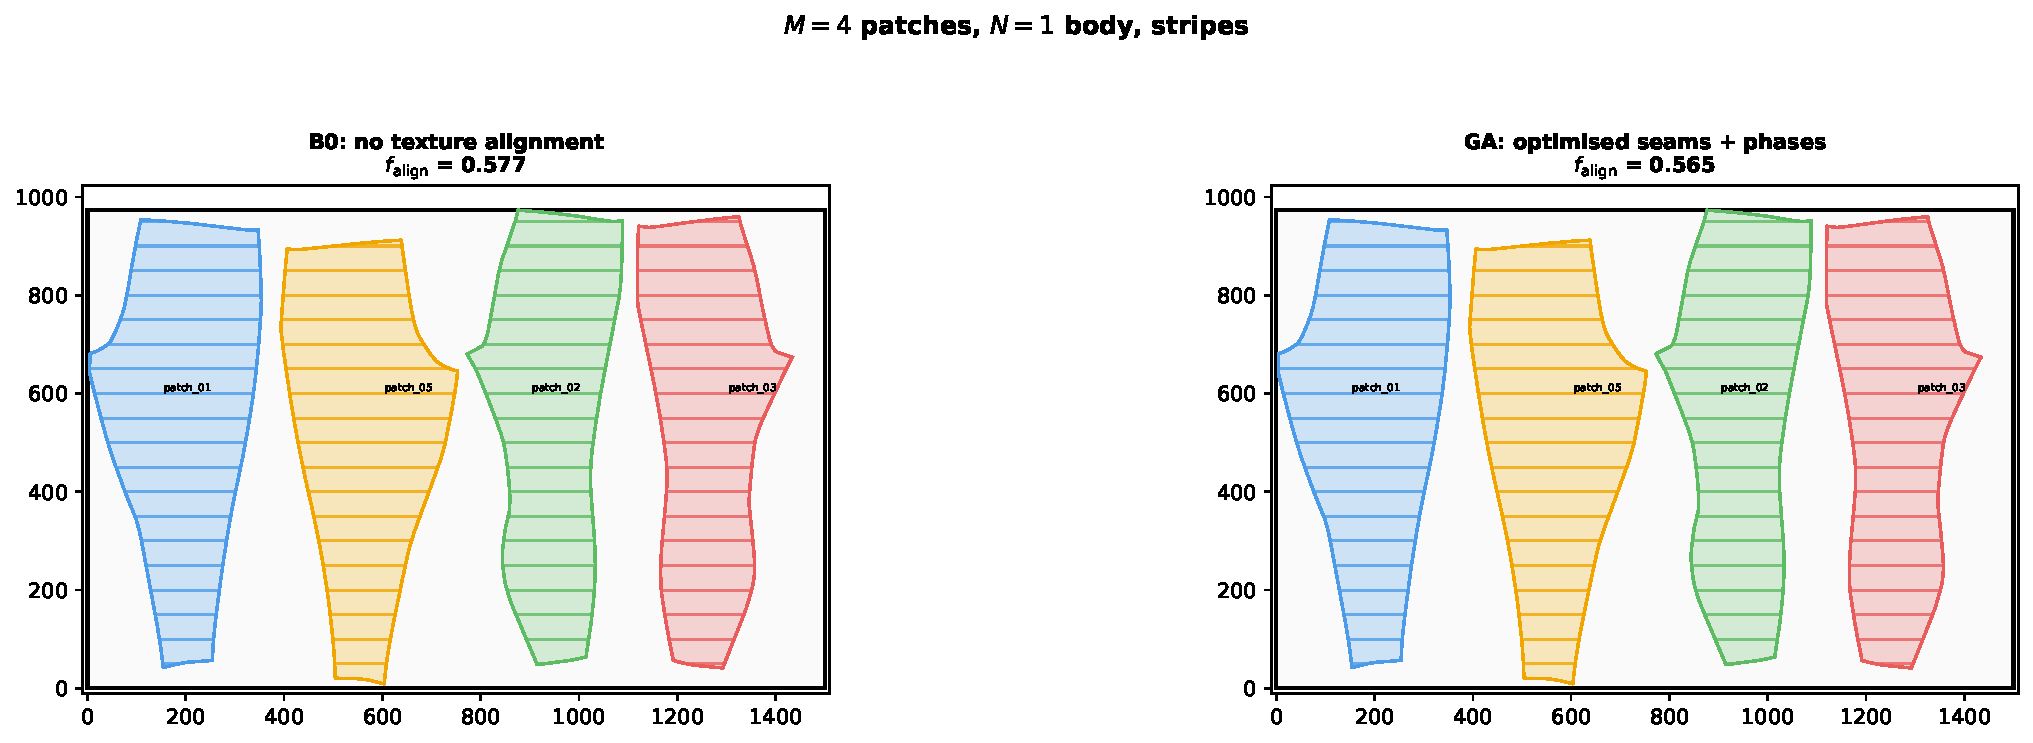
\includegraphics[width=\linewidth]{comparison}
\caption{
  Nesting layout for the pants garment ($M=4$, $N=1$, stripes).
  Left: B0 baseline ($\boldsymbol{\kappa}=\mathbf{0}$, no texture alignment).
  Right: GA result with optimised phase offsets.
  Stripe lines within patches show how the GA shifts texture phases to
  improve alignment across seam boundaries.
}
\label{fig:comparison}
\end{figure}

\paragraph{Convergence and landscape validation.}
Figure~\ref{fig:convergence} reports the best-so-far weighted fitness
$F_\Sigma$ per generation for each body count, and serves as empirical
validation of the landscape analysis in Section~\ref{sec:ea}.
Three predictions from that analysis are testable from the convergence
data.
First, the $\boldsymbol{\delta}$ landscape is piecewise-constant over
Voronoi plateaus, so improvements should appear as discrete jumps when a
mutation crosses a cell boundary rather than as smooth descent.
Second, consecutive improvements should be separated by extended stagnant
stretches where most mutations fall inside the current plateau.
Third, the magnitude of each jump should be non-trivial because crossing a
plateau boundary corresponds to a qualitatively different LSCM flattening,
not an infinitesimal perturbation.
All three predictions hold: across all body counts and seeds, improvements
are concentrated in roughly $3$--$7$ of $20$ generations$^\dagger$, with
total drops of $14$--$29\%$ in $F_\Sigma$, matching the step structure
predicted by the Voronoi tessellation.
This is not a weakness of the optimiser: it is a structural property of
the decision variable $\boldsymbol{\delta}$ under the mesh-vertex snap,
and the population-based search is what allows the optimiser to cross
plateau boundaries at all, since any single-point local search would halt
the first time a mutation failed to improve fitness.
% TODO: replace 3-7 and 14-29 with final 10-seed numbers once runs complete

\begin{figure}[t]
\centering
\includegraphics[width=\linewidth]{convergence}
\caption{
  Best-so-far $F_\Sigma$ vs.\ generation for the onesie garment,
  median and interquartile range over 10 seeds per body count $N$.
  Improvements are concentrated in a small number of generations and
  appear as discrete jumps separated by stagnant stretches, directly
  reflecting the Voronoi tessellation of the $\boldsymbol{\delta}$
  landscape (Section~\ref{sec:ea}): mutations that do not cross a cell
  boundary produce zero fitness change, and each jump corresponds to a
  qualitatively different LSCM flattening.
  $^\dagger$Placeholder; to be replaced with final 10-seed results.
}
\label{fig:convergence}
\end{figure}

% ---------------------------------------------------------------------------
\subsection{Qualitative Results}
\label{sec:qualitative}

Figure~\ref{fig:wallpaper_groups} shows the GA result rendered on the
sleeveless shirt for all eight supported wallpaper groups.
Each garment was optimised independently with the corresponding symmetry
group, demonstrating that the method correctly adapts seam placement and
phase offsets to the specific symmetry structure of each pattern.
Stripe-like groups (PM, PG, PMG, PGG) produce clearly directed motifs that
continue coherently across seam lines, while rotationally symmetric groups
(P4, P4M) yield more isotropic patterns that are inherently less sensitive
to seam placement but still benefit from phase alignment.

\begin{figure}[t]
\centering
\includegraphics[width=\linewidth]{wallpaper_groups}
\caption{
  GA-optimised sleeveless shirt rendered with all eight supported wallpaper
  groups.
  From left to right, top row: stripes (PM), diagonal stripes (PM),
  grid (PMM), pinwheel (P4).
  Bottom row: polka dots (P4M), herringbone (PG), chevron (PMG),
  brick bond (PGG).
  Each result uses the best individual found by the GA in a single run
  ($N=1$ body, pop=20, 5 generations).
}
\label{fig:wallpaper_groups}
\end{figure}

% ---------------------------------------------------------------------------

\section{Conclusion}
\label{sec:conclusion}

We formulated garment pattern layout as a joint optimisation over seam
positions, fabric efficiency, and texture alignment, with an explicit
fit-preservation guard, and demonstrated its solvability with a
mixed-integer evolution strategy.
By optimising seam positions directly on the 3D body mesh, all pattern
modifications are grounded in body geometry, making fit deviation an
explicit and measurable quantity.
A global phase alignment stage and discrete texture phase offsets per patch
exploit the full periodic symmetry of the fabric, modelled across eight
wallpaper groups including those with glide-reflection symmetry.
Systematic ablation decomposes the GA's advantage into three individually
attributable components: $\boldsymbol{\delta}$ search provides the
largest single improvement (12\% over the best $\boldsymbol{\kappa}$-only
baseline), evolutionary operators exploit the sparse
$\boldsymbol{\delta}$ landscape more effectively than random search
(${\sim}$3\%), and $\boldsymbol{\kappa}$ mutation contributes a further
${\sim}$6\% by reaching global phase reconfigurations inaccessible to
Stage~2 alone.
Experiments on three garment types ($M \in \{2, 4, 11\}$) with up to
2{,}200 pattern pieces demonstrate consistent improvement in texture
alignment over all baselines including random search at matched
evaluation budget.

\paragraph{Limitations and future work.}
The nesting engine uses a bottom-left heuristic; substituting an
NFP-based solver~\cite{MartinezSykoraACRO22} could improve fabric
utilisation without affecting the other contributions.
Approximately 55--60\,\% of candidate $\boldsymbol{\delta}$ configurations
fail during geometry processing (geodesic or LSCM singularities),
receiving death-penalty fitness; more robust geometry processing or
adaptive step-size control would improve effective population utilisation.
The discrete Voronoi structure of the $\boldsymbol{\delta}$ landscape
(Section~\ref{sec:ea}) causes many neutral mutations; adaptive step-size
control or landscape-aware operators could accelerate convergence.
Finally, extending the framework to multiple body shapes and sizes within
a single fabric roll is a natural next step toward industrial deployment.


\bibliographystyle{splncs04}
\bibliography{refs}

\end{document}
